\documentclass{standalone}
\usepackage{tikz}
\usepackage{xparse}
\definecolor{digit-0}{HTML}{0d0d0f}
\definecolor{digit-1}{HTML}{7d4b25}
\definecolor{digit-2}{HTML}{fd0017}
\definecolor{digit-3}{HTML}{fd9721}
\definecolor{digit-4}{HTML}{fefe32}
\definecolor{digit-5}{HTML}{10af52}
\definecolor{digit-6}{HTML}{0f4fcd}
\definecolor{digit-7}{HTML}{9810fc}
\definecolor{digit-8}{HTML}{a5a5a5}
\definecolor{digit-9}{HTML}{ffffff}
\definecolor{tolerance-0.1}{HTML}{9810fc}
\definecolor{tolerance-0.5}{HTML}{10af52}
\definecolor{tolerance-1}{HTML}{7d4b25}
\definecolor{tolerance-5}{HTML}{ffd600}
\definecolor{tolerance-10}{HTML}{bfbfbf}
\begin{document}
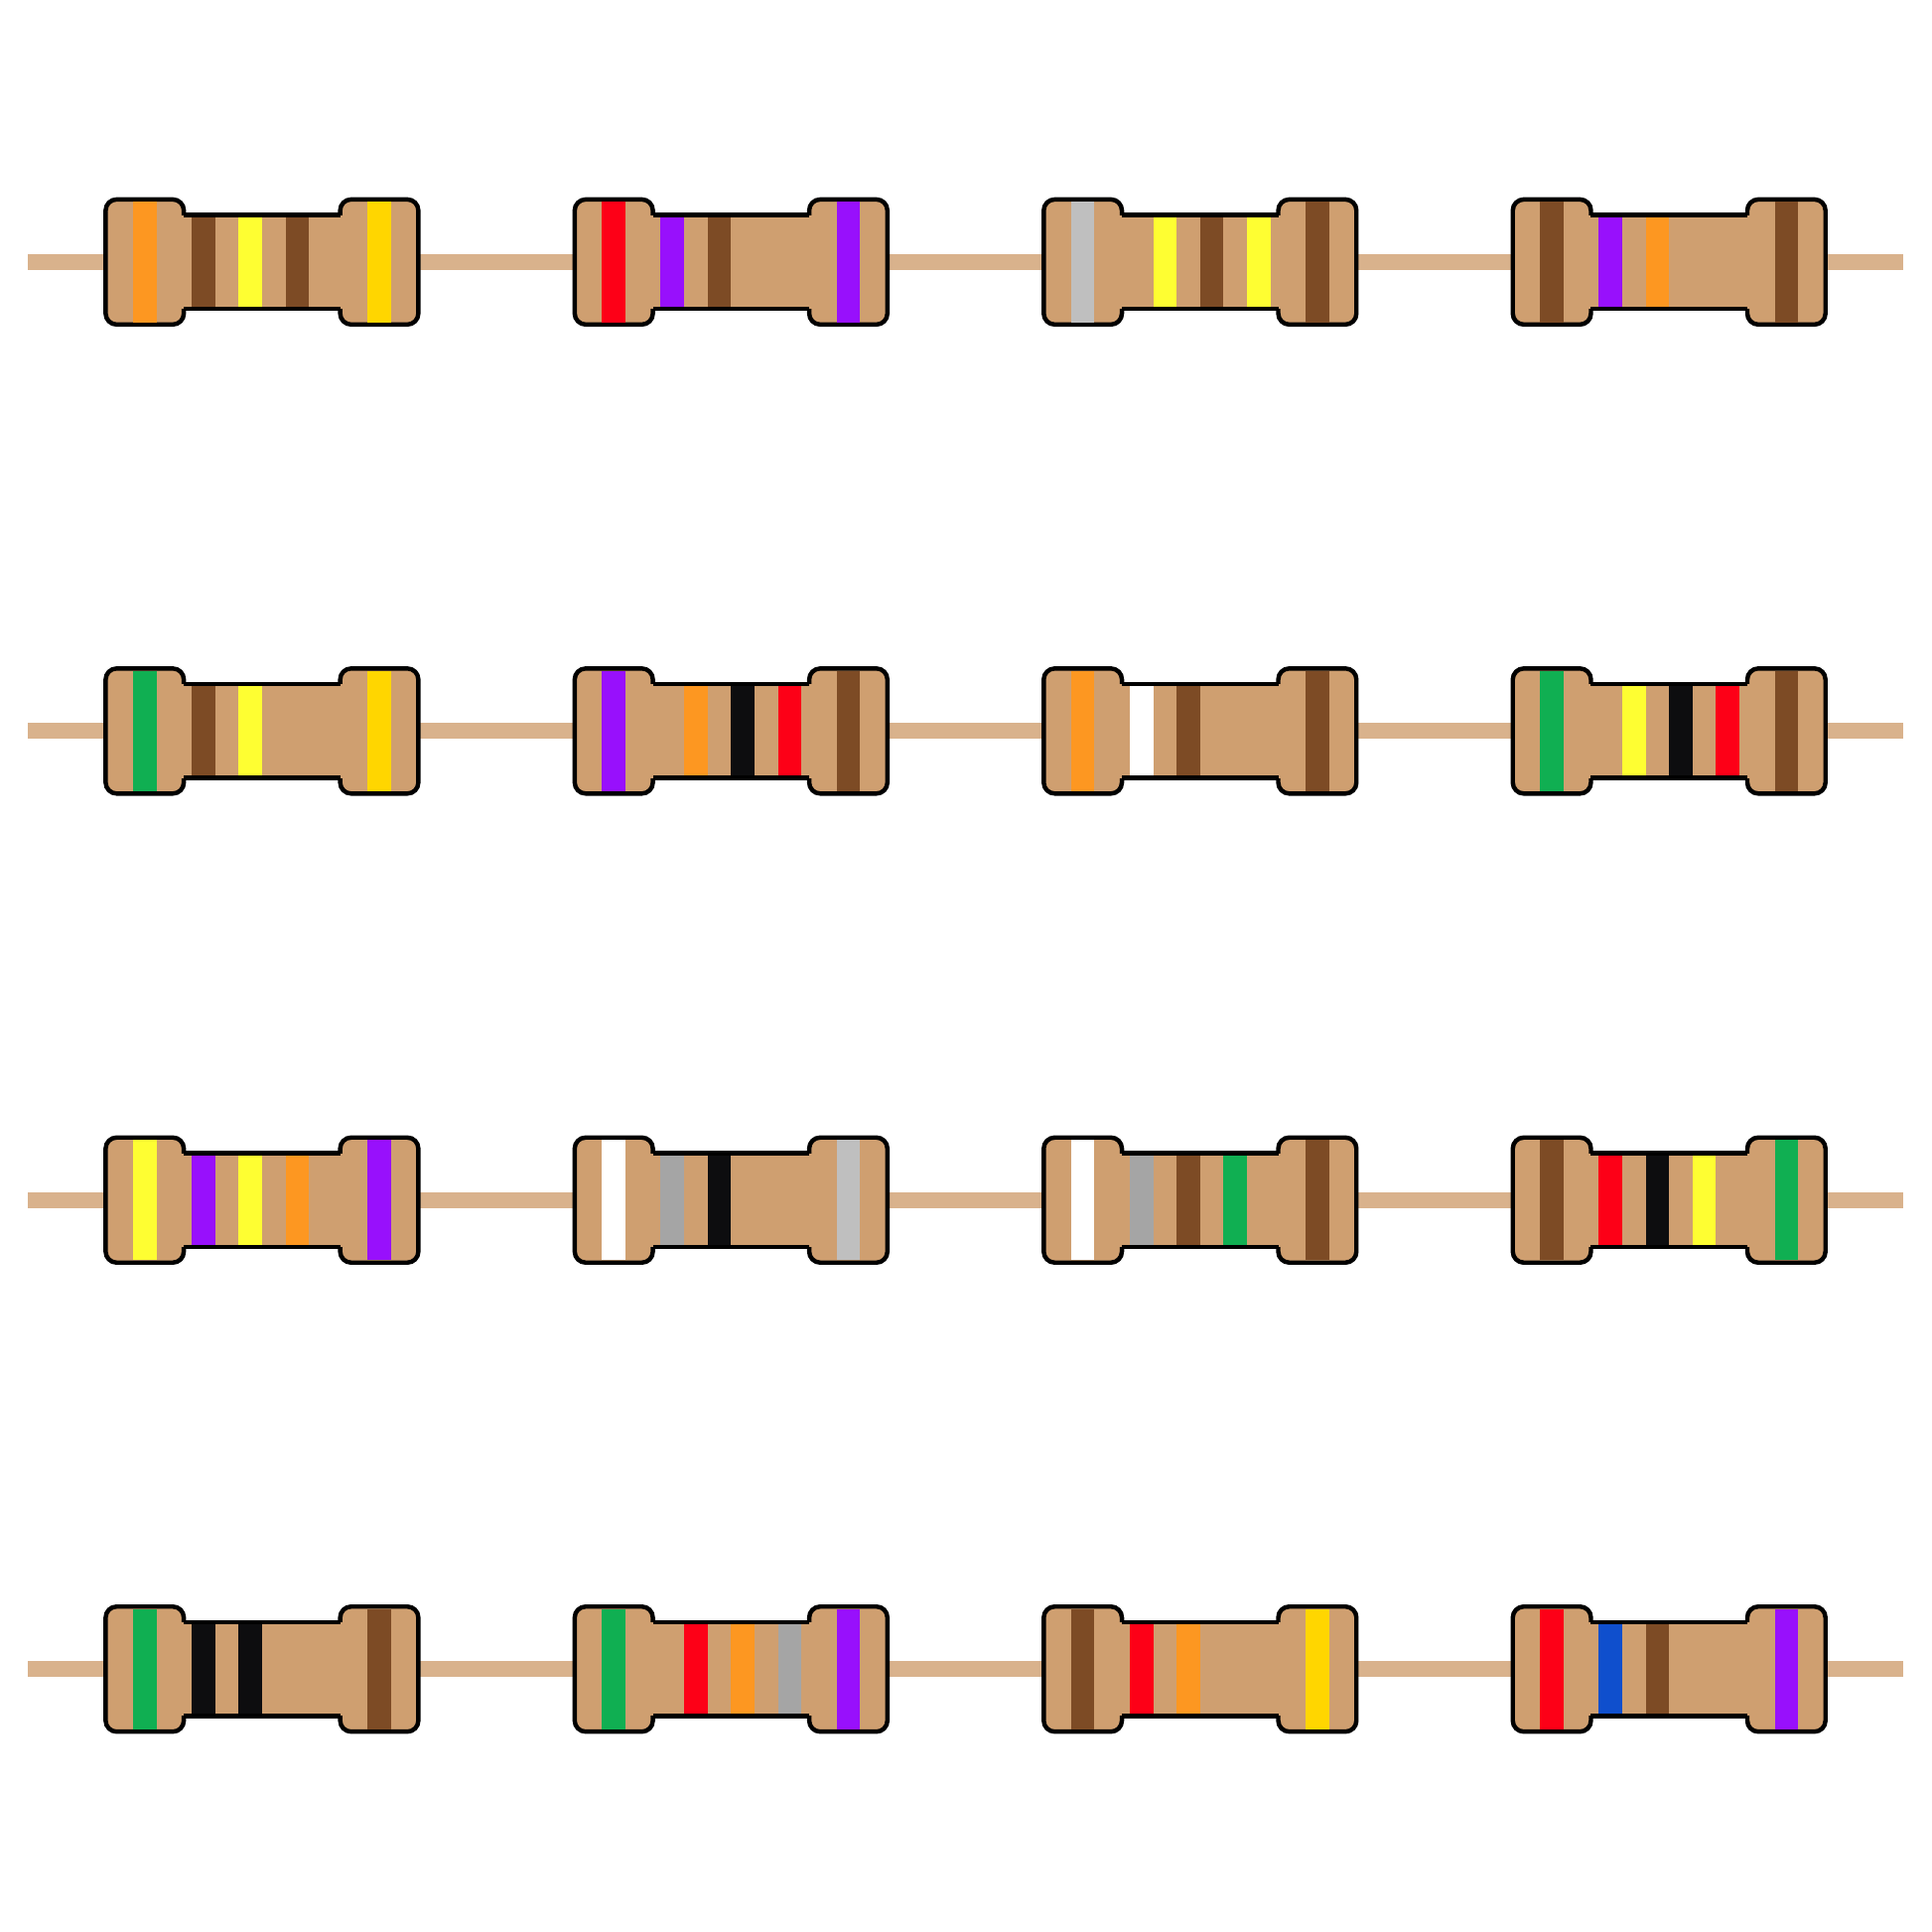
\begin{tikzpicture}
	\NewDocumentCommand{\res}{mmomm}{
		\fill[color=brown!60](-3,-.1)rectangle(3,.1);
		\draw[ultra thick,fill=brown!75,rounded corners](-2,-.8)rectangle(-1,.8);
		\draw[ultra thick,fill=brown!75,rounded corners](2,-.8)rectangle(1,.8);
		\fill[color=brown!75](-1.1,-.6)rectangle(1.1,.6);
		\draw[ultra thick](-1,-.6)--(1,-.6) (-1,.6)--(1,.6);
		\fill[color=digit-#1](-1.65,-.77)rectangle(-1.35,.77);
		\fill[color=digit-#2](-.9,-.57)rectangle(-.6,.57);
		\IfNoValueTF{#3}{
			\fill[color=digit-#4](-.3,-.57)rectangle(0,.57);
		}{
			\fill[color=digit-#3](-.3,-.57)rectangle(0,.57);
			\fill[color=digit-#4](.3,-.57)rectangle(.6,.57);
		}
		\fill[color=tolerance-#5](1.35,-.77)rectangle(1.65,.77);
	}
	\draw[draw=none](-3,-3)rectangle(21,21);
	\scoped[shift={(0,0)},rotate=0]{\res{5}{0}{0}{1}};
	\scoped[shift={(6,0)},rotate=180]{\res{7}{8}[3]{2}{0.5}};
	\scoped[shift={(12,0)},rotate=0]{\res{1}{2}{3}{5}};
	\scoped[shift={(18,0)},rotate=0]{\res{2}{6}{1}{0.1}};
	\scoped[shift={(0,6)},rotate=0]{\res{4}{7}[4]{3}{0.1}};
	\scoped[shift={(6,6)},rotate=0]{\res{9}{8}{0}{10}};
	\scoped[shift={(12,6)},rotate=0]{\res{9}{8}[1]{5}{1}};
	\scoped[shift={(18,6)},rotate=0]{\res{1}{2}[0]{4}{0.5}};
	\scoped[shift={(0,12)},rotate=0]{\res{5}{1}{4}{5}};
	\scoped[shift={(6,12)},rotate=180]{\res{1}{2}[0]{3}{0.1}};
	\scoped[shift={(12,12)},rotate=0]{\res{3}{9}{1}{1}};
	\scoped[shift={(18,12)},rotate=180]{\res{1}{2}[0]{4}{0.5}};
	\scoped[shift={(0,18)},rotate=0]{\res{3}{1}[4]{1}{5}};
	\scoped[shift={(6,18)},rotate=0]{\res{2}{7}{1}{0.1}};
	\scoped[shift={(12,18)},rotate=180]{\res{1}{4}[1]{4}{10}};
	\scoped[shift={(18,18)},rotate=0]{\res{1}{7}{3}{1}};
\end{tikzpicture}
\end{document}
